\documentclass[cs4size,a4paper,10pt]{ctexart}   

\linespread{1.5}
\usepackage{geometry}%用于设置上下左右页边距
	\geometry{left=2.5cm,right=2.5cm,top=3.2cm,bottom=2.7cm}
\usepackage{xeCJK,amsmath,paralist,enumerate,booktabs,multirow,graphicx,subfig,setspace,listings,lastpage,hyperref}
\usepackage{amsthm, amssymb, bm, color, framed, graphicx, hyperref, mathrsfs}
\usepackage{mathrsfs}  
	\setlength{\parindent}{2em}
	\lstset{language=Matlab}%
\usepackage{fancyhdr}
\usepackage{graphicx}
\usepackage{subfloat}
\usepackage{listings}
\usepackage{xcolor}
\usepackage{float}
\usepackage{paralist}
\usepackage{setspace}
\usepackage{titlesec}
\usepackage{enumitem}
\usepackage{hyperref}



\hypersetup{
	colorlinks=true,
	linkcolor=black
}

\setenumerate{partopsep=0pt,topsep=0pt}
\setitemize{itemsep=0pt,partopsep=0pt,topsep=0pt}

\titlespacing*{\section}{0pt}{3pt}{3pt}
\titlespacing*{\subsection}{0pt}{2pt}{2pt}
\titlespacing*{\subsubsection}{0pt}{1pt}{1pt}
\titlespacing*{\paragraph}{0pt}{0pt}{0pt}

\ctexset{secnumdepth=4,tocdepth=4}
\setlength{\parindent}{0pt}
\setstretch{1.2}


\setCJKmainfont[BoldFont={FZHei-B01},ItalicFont={FZKai-Z03}]{FZShuSong-Z01} 
\setCJKsansfont[BoldFont={FZHei-B01}]{FZKai-Z03} 
\setCJKmonofont[BoldFont={FZHei-B01}]{FZFangSong-Z02}
\setCJKfamilyfont{zhsong}{FZShuSong-Z01} 
\setCJKfamilyfont{zhhei}{FZHei-B01} 
\setCJKfamilyfont{zhkai}[BoldFont={FZHei-B01}]{FZKai-Z03} 
\setCJKfamilyfont{zhfs}[BoldFont={FZHei-B01}]{FZFangSong-Z02} 
\renewcommand*{\songti}{\CJKfamily{zhsong}} 
\renewcommand*{\heiti}{\CJKfamily{zhhei}} 
\renewcommand*{\kaishu}{\CJKfamily{zhkai}} 
\renewcommand*{\fangsong}{\CJKfamily{zhfs}}


\definecolor{mKeyword}{RGB}{0,0,255}          % bule
\definecolor{mString}{RGB}{160,32,240}        % purple
\definecolor{mComment}{RGB}{34,139,34}        % green
\definecolor{mNumber}{RGB}{128,128,128} 

\lstdefinestyle {njulisting} {
	basewidth = 0.5 em,
	lineskip = 3 pt,
	basicstyle = \small\ttfamily,
	% keywordstyle = \bfseries,
	commentstyle = \itshape\color{gray}, 
	basicstyle=\small\ttfamily,
	keywordstyle={\color{mKeyword}},     % sets color for keywords
	stringstyle={\color{mString}},       % sets color for strings
	commentstyle={\color{mComment}},     % sets color for comments
	numberstyle=\tiny\color{mNumber},
	numbers = left,
	captionpos = t,
	breaklines = true,
	xleftmargin = 2 em,
	xrightmargin = 2 em,
	frame=tlrb,
	tabsize=4
}

\lstset{
style = njulisting, % 调用上述样式 
flexiblecolumns % 允许调整字符宽度
}


%================= 基本格式预置 ===========================
\usepackage{fancyhdr}
\pagestyle{fancy}
\lhead{\textsc{Operating System}}
\rhead{第三章\ 存储管理}
\cfoot{\thepage}
\renewcommand{\headrulewidth}{0.4pt}
\renewcommand{\theenumi}{(\arabic{enumi})}
\CTEXsetup[format={\bfseries\zihao{-3}}]{section}
\CTEXsetup[format={\bfseries\zihao{4}}]{subsection}
\CTEXsetup[format={\bfseries\zihao{-4}}]{subsubsection}


\renewcommand{\contentsname}{目录}  
\begin{document}

	\begin{center}
		{\huge\textbf{第三章\ 存储管理}}
	\end{center}
	%---------目录---------% 
	\pagenumbering{Roman}
	\tableofcontents
	\clearpage

 	%---------正文---------% 
	\pagenumbering{arabic}
	\setcounter{page}{1}
	\setlength{\parskip}{0.65em}
	
	\section{存储管理基础}
	\subsection{存储管理的主要模式}
	\subsubsection{逻辑地址与物理地址}
	逻辑地址,又称相对地址。目标代码程序存放在磁盘文件中,由于程序在主存中的位置不可预知,程序地址空间中的地址总是相对于某个基准(通常为 0)开始连续编号

	逻辑地址有两种形式
	\begin{itemize}
		\item 一维逻辑地址:所有程序和数据组成一维的逻辑地址
		\item 二维逻辑地址:一个用户程序可以设计成多个段,每个段都从 0 开始编址
		\begin{itemize}
			\item 二维逻辑地址引入段式程序设计的概念
			\begin{itemize}
				\item 一个程序可以包含若干代码段、数据段、堆栈段
				\item 用户可以自己应用段覆盖技术扩充内存空间使用量
				\begin{itemize}
					\item 用户在程序设计时包括主程序段、堆栈段、多个子程序段和数据段,而执行程序时只调入主程序段、堆栈段和需要的子程序段和数据段
					\item 由程序设计者预先设计的代码动态决定哪些段调入主存
					\item 这一技术是程序设计技术,不是操作系统存储管理的功能
				\end{itemize}
			\end{itemize}
		\end{itemize}
	\end{itemize}
	
	物理地址,又称绝对地址,即程序执行所使用的地址空间
	\begin{itemize}
		\item 处理器执行指令时按照物理地址进行
	\end{itemize}


	\subsubsection{主存的复用方式}
	多道程序设计需要多个进程来划分使用主存

	主存复用有分区复用和页框复用两种方式
	\begin{itemize}
		\item 分区复用是指将主存划分为多个固定或可变尺寸的分区
		\begin{itemize}
			\item 一个程序或一个程序段占用一个分区
		\end{itemize}
		\item 页框复用是指将主存划分成多个固定大小的页框(页架或主存物理块)
		\begin{itemize}
			\item 一个程序或一个程序段根据页框大小自动划分为页面,进而占用多个页框
		\end{itemize}
	\end{itemize}

	存储管理的基本模式
	\begin{itemize}
		\item 单连续存储管理:一维逻辑地址空间的程序占用一个主存固定分区或可变分区
		\item 段式存储管理:段式二维逻辑地址空间的程序占用多个主存可变分区
		\item 页式存储管理:一维逻辑地址空间的程序占用多个主存页架区
		\item 段页式存储管理:段式二维逻辑地址空间的程序占用多个主存页架区
	\end{itemize}
	\begin{figure}[H]
		\centering
		\includegraphics[width=0.9\textwidth]{img/3.1.1.2}
	\end{figure}

	\subsection{存储管理的功能}
	\subsubsection{地址转换}
	地址转换又称重定位,即把逻辑地址转换成绝对地址
	\begin{itemize}
		\item 静态重定位:在程序装入内存时进行地址转换
		\begin{itemize}
			\item 由装入程序执行,早期小型操作系统使用
		\end{itemize}
		\item 动态重定位(主流):在 CPU 执行程序时进行地址转换
		\begin{itemize}
			\item 从效率出发,依赖硬件地址转换机制
		\end{itemize}
	\end{itemize}

	\subsubsection{主存空间的分配与去配}
	\begin{itemize}
		\item 分配:进程装入主存时,存储管理软件进行具体的主存分配操作,并设置一个表格记录主存空间的分配情况
		\item 去配:当某个进程撤离或主动归还主存资源时,存储管理软件要收回它所占用的全部或者部分存储空间,调整主存分配表信息
	\end{itemize}

	\subsubsection{主存空间的共享}
	多个进程共享主存包括两个层次的概念:
	\begin{itemize}
		\item 多个进程共享主存储器资源
		\begin{itemize}
			\item 多道程序设计技术使若干个程序同时进入主存储器,各自占用一定数量的存储空间,共同使用一个主存储器
		\end{itemize}
		\item 多个进程共享主存储器的某些区域
		\begin{itemize}
			\item 若干个协作进程有共同的主存程序块或者主存数据块
		\end{itemize}
	\end{itemize}


	\subsubsection{存储保护}
	为避免主存中的多个进程相互干扰,必须对主存中的程序和数据进行保护
	\begin{itemize}
		\item 私有主存区中的信息:可读可写
		\item 公共区中的共享信息:根据授权
		\item 非本进程信息:不可读写
	\end{itemize}
	存储保护需要软硬件协同完成
	\begin{itemize}
		\item CPU 检查是否允许访问,不允许则产生地址保护异常
		\item 由操作系统进行相应处理
	\end{itemize}


	\subsubsection{主存空间的扩充}
	存储扩充:把磁盘作为主存扩充,只把部分进程或进程的部分内容装入内存
	\begin{itemize}
		\item 对换技术:把部分不运行的进程调出
		\item 虚拟技术:只调入进程的部分内容
	\end{itemize}
	这一工作需要软硬件协作完成
	\begin{itemize}
		\item 对换进程决定对换,硬件结构调入
		\item CPU 处理到不在主存的地址,发出虚拟地址异常,操作系统将其调入,重新执行指令
	\end{itemize}

	\subsection{虚拟存储器概述}
	\subsubsection{虚拟存储器思想的提出}
	\begin{itemize}
		\item 主存容量限制带来诸多不便
		\begin{itemize}
			\item 用户编写程序必须考虑主存容量限制
			\item 多道程序设计的道数受到限制
		\end{itemize}
		\item 用户编程行为分析
		\begin{itemize}
			\item 全面考虑各种情况,执行时有互斥性
			\item 顺序性和循环性等空间局部性行为
			\item 某一阶段执行的时间局部性行为
		\end{itemize}
		\item 因此可以考虑部分调入进程内容
	\end{itemize}

	\subsubsection{虚拟存储器的基本思想}
	存储管理把进程全部信息放在辅存中,执行时先将其中一部分装入主存,以后根据执行行为\textbf{随用随调入}

	如主存中没有足够的空闲空间,存储管理需要根据执行行为把主存中暂时不用的信息\textbf{调出}到辅存上去


	\subsubsection{虚拟存储器的实现思路}
	需要建立与自动管理两个地址空间
	\begin{itemize}
		\item (辅存)虚拟地址空间:容纳进程装入
		\item (主存)实际地址空间:承载进程执行
	\end{itemize}
	对于用户,计算机系统具有一个容量大得多的主存空间,即\textbf{虚拟存储器}

	虚拟存储器是一种地址空间扩展技术,通常意义上对用户编程是透明的,除非用户需要进行高性能的程序设计
	\begin{figure}[H]
		\centering
		\includegraphics[width=0.6\textwidth]{img/3.1.3.3}
	\end{figure}

	\subsection{存储管理的硬件支撑}
	\subsubsection{存储器层次}
	\begin{figure}[H]
		\centering
		\includegraphics[width=0.6\textwidth]{img/3.1.4.1.1}
	\end{figure}
	\begin{itemize}
		\item 越处于顶端,访问速度越快,容量越小,单位字节价格会越高。根据实际情况,选择使用什么样的存储器
		\begin{itemize}
			\item 寄存器、缓存和内存属于操作系统存储管理的范畴,掉电后信息丢失
			\item 磁盘和磁带属于稳健管理和设备管理的管辖对象,信息永久保存
		\end{itemize}
		\item 可执行程序必须被保存在内存中,与设备交换的信息也依托于内存地址空间
		\item 由于程序处理数据时存在顺序性和局部性,故执行时仅需调入当前运行使用的一部分,其他部分待需要时再逐步调入
	\end{itemize}


	\subsubsection{存储管理涉及的存储对象}
	\begin{itemize}
		\item 存储管理是操作系统管理主存储器的软件部分
		\item 为获得更好的处理性能,部分主存程序与数据(特别是关键性能数据)被调入 Cache,存储管理需要对其进行管理, 甚至包括对联想存储器的管理
		\item 为获得更大的虚拟地址空间,存储管理需要对存放在硬盘、固态硬盘、甚至网络硬盘上的虚拟存储器文件进行管理
	\end{itemize}


	\subsubsection{高速缓存存储器Cache}
	Cache 是介于 CPU 和主存储器间的高速小容量存储器,由静态存储芯片 SRAM 组成,容量较小但比主存 DRAM 技术更加昂贵而快速, 接近于 CPU 的速度

	CPU 往往需要重复读取同样的数据块,Cache 的引入与缓存容量的增大,可以大幅提升 CPU 内部读取数据的命中率, 从而提高系统性能

	高速缓冲存储器通常由高速存储器、联想存储器、地址转换部件、替换逻辑等组成
	\begin{itemize}
		\item 联想存储器:根据内容进行寻址的存储器
		\item 地址转换部件:通过联想存储器建立目录表以实现快速地址转换,命中时直接访问 Cache,未命中时从内存读取放入 Cache
		\item 替换逻辑部件:在缓存已满时按一定策略进行数据块替换,并修改地址转换部件
	\end{itemize}

	高速缓存存储器的组织
	\begin{itemize}
		\item 由于 CPU 芯片面积和成本,Cache 很小
		\item 根据成本控制,划分为 L1、L2、L3三级
		\begin{itemize}
			\item L1 Cache:分为数据缓存和指令缓存,内置,成本最高,对 CPU 的性能影响最大,通常在 32KB$\sim$256K 之间
			\item L2 Cache:分内置和外置两种,后者性能低一些,通常在 512KB$\sim$8MB 之间
			\item L3 Cache:多为外置,在游戏和服务器领域有效,但对很多应用来说,总线改善比设置 L3 更加有利于提升系统性能
		\end{itemize}
	\end{itemize}
	\begin{figure}[H]
		\centering
		\includegraphics[width=0.7\textwidth]{img/3.1.4.3}
	\end{figure}


	\subsubsection{存储管理的硬件支持}
	\begin{figure}[H]
		\centering
		\includegraphics[width=0.6\textwidth]{img/3.1.4.4}
	\end{figure}
	\begin{itemize}
		\item 鉴于程序执行与数据访问的局部性原理,存储管理软件使用 Cache 可以大幅度提升程序执行效率
		\item 动态重定位、存储保护等,若无硬件支撑在效率上是无意义的,即无实现价值
		\item 无虚拟地址中断,虚拟存储器无法实现
		\item 无页面替换等硬件支撑机制,虚拟存储器在效率上是无意义的
	\end{itemize}

	\section{单连续分区存储管理}
	单连续分区存储管理是指每个进程占用物理上完全连续的存储空间,它可以细分为三种:
	\begin{itemize}
		\item 单用户连续分区存储管理
		\item 固定分区存储管理
		\item 可变分区存储管理
	\end{itemize}

	\subsection{单用户连续分区存储管理}
	\begin{figure}[H]
		\centering
		\includegraphics[width=0.6\textwidth]{img/3.2.1}
	\end{figure}

	\begin{itemize}
		\item 主存区域划分为\textbf{系统区}与\textbf{用户区}
		\item 设置一个\textbf{栅栏寄存器}界分两个区域,硬件用它在执行时进行存储保护
		\item 一般采用静态重定位进行地址转换
		\item 硬件实现代价低,适用于单用户单任务操作系统,如 DOS
	\end{itemize}

	\subsection{固定分区存储管理}
	固定分区的基本思想是:内存空间被划分为数目固定不变的分区,各分区大小不等,每个分区只装入一个作业,若多个分区中都装有作业,则它们都可以并发执行

	为了管理各分区的分配和使用情况,需要设置一张主存分配表,记录主存中划分的分区及其使用情况
	\begin{itemize}
		\item 主存分配表指出各分区的起始地址和长度
		\item 利用占位标志符指示此分区是否被使用
		\begin{itemize}
			\item 当其值为 0 时表明此分区尚未被使用
		\end{itemize}
		\item 主存分配时选择那些未被占用但是容量足够的分区,填入占用此分区的作业名
		\item 当分区中的程序执行结束归还主存区时,相应分区的占用标志被置为 0,其占用的分区又可被重新分配使用
	\end{itemize}
	\textbf{例}:如下主存分配表中,第 2、5 分区分别被作业 $Job_1$ 和 $Job_2$ 占用,其余分区空闲
	\begin{table}[H]
		\centering
		\begin{tabular}{|c|c|c|c|}
		\hline
		分区号 & 起始地址  & 长度    & 占用标志    \\ \hline
		1   & 8 KB  & 8 KB  & 0       \\ \hline
		2   & 16 KB & 16 KB & $Job_1$ \\ \hline
		3   & 32 KB & 16 KB & 0       \\ \hline
		4   & 48 KB & 16 KB & 0       \\ \hline
		5   & 64 KB & 32 KB & $Job_2$ \\ \hline
		6   & 96 KB & 32 KB & 0       \\ \hline
		\end{tabular}
		\end{table}

		固定分区存储管理一般采用动态地址重定位

		下图给出了固定分区的地址转换与存储保护机制,图中所示为一种上限/下限寄存器实现方案
		\begin{itemize}
			\item 每个分区有上限和下限,分别界定了分区的结束地址和起始地址
			\item 当进程占有 CPU 运行时,它就占有了 CPU 现场的上限/下限奇存器
			\item 把下限地址与逻辑地址相加得到绝对地址,将绝对地址与上限地址进行比较
			\begin{itemize}
				\item 如果超越了这个范围则产生越界中断进行存储保护
				\item 否则就根据该绝对地址访问具体的进程用户空问的存储单元
			\end{itemize}
		\end{itemize}
		\begin{figure}[H]
			\centering
			\includegraphics[width=0.65\textwidth]{img/3.2.2}
		\end{figure}

		固定分区存储管理的缺点
		\begin{itemize}
			\item 由于预先规定分区大小,大作业可能无法装入,用户程序设计不方便
			\item 主存空间利用率不高,作业很少能恰好填满分区,从而出现分区内的碎片,称为主存内零头,也称为内部碎片
			\item 如果一个进程在运行过程中要求动态扩充主存空间,采用固定分区相当困难
			\item 分区数目是在系统初启时确定的,这就会限制允许加载的多道运行程序的道数,特别不适合分时系统交互型用户及主存需求变化很大的情形
		\end{itemize}

		\subsection{可变分区存储管理}
		可变分区存储管理按进程的内存需求来动态划分分区
		\begin{itemize}
			\item 创建一个进程时,根据进程所需主存量查看主存中是否有足够的空闲空间
			\begin{itemize}
				\item 若有,则按需要量分割一个分区
				\item 若无,则令该进程等待主存资源
			\end{itemize}
			\item 由于分区大小按照进程实际需要量来确定,因此分区个数是随机变化的
		\end{itemize}
		\begin{figure}[H]
			\centering
			\includegraphics[width=0.65\textwidth]{img/3.2.3}
		\end{figure}
		
		\subsubsection{主存空间的分配和去配}
		\begin{figure}[H]
			\centering
			\includegraphics[width=0.6\textwidth]{img/3.2.3.1}
		\end{figure}

		可变分区方式的内存回收会导致内存空间的转换,作业 $X$ 撤离后有且仅有如上 4 种情况

		常用的可变分区主存分配算法有以下几种:
		\begin{itemize}
			\item 最先适应分配算法:
			\begin{itemize}
				\item 最先适应就是从上向下查找,找到第一块区域放进去,将剩下的区域分割后仍作为空闲区
				\item 有利于大作业装入,但也使得内存低地址和高地址两端的分区利用不均衡,回收分区麻烦
			\end{itemize}
			\item 邻近适应分配算法:
			\begin{itemize}
				\item 从上次查找结束的地方开始执行最先适应分配算法
				\item 缩短平均查找时间,且存储空间利用率更均衡,不会使得小空闲区集中在内存一侧
			\end{itemize}
			\item 最优适应分配算法:
			\begin{itemize}
				\item 每次都是分配最接近需要使用大小的部分,会生成很多很小的内存内零头
				\item 通常会将空闲区按照长度递增顺序排列,等同于最先适应分配算法,查找时间最长
			\end{itemize}
			\item 最坏适应分配算法:
			\begin{itemize}
				\item 每次都是挑选最大的一块区域进行分配
				\item 有利于中小型作业
				\item 可把空闲区按长度递减顺序排列,等同于最先适应分配算法
			\end{itemize}
			\item 快速适应分配算法:
			\begin{itemize}
				\item 为经常用到的长度的空闲区设立单独的空闲区链表,查找非常快速
				\item 归还内存空间时和邻近空闲区的合并复杂且耗时
			\end{itemize}
		\end{itemize}

		\subsubsection{地址转换与存储保护}
		\begin{figure}[H]
			\centering
			\includegraphics[width=0.6\textwidth]{img/3.2.3.2}
		\end{figure}
		硬件实现机制与动态重定位

		进程的程序和数据的地址由硬件完成
		\begin{itemize}
			\item 基址寄存器:分配进程的起始地址
			\item 限长寄存器:进程占用的连续存储空间的长度
		\end{itemize}

		\subsubsection{可变分区的主存外零头}
		固定分区方式会产生内存内零头;可变分区方式也会随着进程的内存分配产生一些小的不可用的内存分区,称为内存外零头
		\begin{itemize}
			\item 最优适配算法最容易产生外零头
			\item 任何适配算法都不能避免产生外零头
		\end{itemize}
		当在未分配区表中找不到足够大的空闲区来装入新的进程时,可以把已在主存中的进程分区连接到一起,使分散的空闲区汇集成片,这就是\textbf{移动技术},也称\textbf{主存紧凑}
		\begin{itemize}
			\item 需要动态地址重定位技术的支撑
			\item 移动技术有极大的系统开销,而且并不是任何时间下都可以进行的,当一道程序正在与设备交换数据时往往不能移动
		\end{itemize}
		\begin{figure}[H]
			\centering
			\includegraphics[width=0.5\textwidth]{img/3.2.3.3.1}
		\end{figure}

		支持移动技术的可变分区存储管理的主存分配算法
		\begin{figure}[H]
			\centering
			\includegraphics[width=0.7\textwidth]{img/3.2.3.3.2}
		\end{figure}

		\subsection{伙伴系统}
		\subsubsection{伙伴系统的实现原理}
		\begin{itemize}
			\item 伙伴系统,又称 buddy 算法,是一种固定分区和可变分区折中的主存管理算法
			\item 基本原理是:任何尺寸为 $2^i$ 的空闲块都可被分为两个尺寸为 $2^{i-1}$ 的空闲块,这两个空闲块称作伙伴,它们可以被合并成尺寸为 $2^i$ 的原先空闲块
			\item 伙伴通过对大块的物理主存划分而获得
			\begin{itemize}
				\item 假如从第 0 个页面开始到第 3 个页面结束的主存
				\item 每次都对半划分,那么第一次划分获得大小为 2 页的伙伴,如 0、 1 和 2、3
				\item 进一步划分,可以获得大小为 1 页的伙伴,例如 0 和 1,2 和 3
			\end{itemize}
		\end{itemize}
		\begin{figure}[H]
			\centering
			\includegraphics[width=0.8\textwidth]{img/3.2.4.1}
		\end{figure}

		类似二叉树的形式进行分配
		\begin{figure}[H]
			\centering
			\includegraphics[width=0.7\textwidth]{img/3.2.4.2}
		\end{figure}

		\subsubsection{Linux伙伴系统}
		\begin{itemize}
			\item 以 \verb|page| 结构为数组元素的 \verb|mem_map[ ]| 数组
			\item 以 \verb|free_area_struct| 结构为数组元素的 \verb|free_area| 数组
			\item 位图数组(bitmap)
		\end{itemize}
		伙伴系统以页框为基本分配单位,内核在很多情况下,需要的主存量远远小于页框大小,为了更经济地使用内核主存资源,引入 SunOS 操作系统中首创的基于伙伴系统的 \textbf{slab分配器}
		\begin{itemize}
			\item 其基本思想是:为经常使用的小对象建立缓存,小对象的申请与释放都通过 slab 分配器来管理,仅当缓存不够用时才向伙伴系统申请更多空间
			\item 优点:充分利用主存,减少内部碎片,对象管理局部化, 尽可能少地与伙伴系统打交道,从而提高效率
		\end{itemize}

		slab 的结构
		\begin{lstlisting}[language=C,keywordstyle=\color{black}]
struct slab{
   struct list_head;          //slab满、半满或空闲链表
   unsigned long colouoff;    //slab着色偏移量
   void * s_mem;              //slab的第一个对象
   unsigned int inuse;        //已分配的对象数
   kmem_bufctl_t free;        //第一个空闲对象
}
		\end{lstlisting}

		\begin{figure}[H]
			\centering
			\includegraphics[width=0.75\textwidth]{img/3.2.4.3}
		\end{figure}
		slab 分配器主要操作
		\begin{itemize}
			\item \verb|kmem_cache_create()| 函数:创建专用 cache,规定对象的大小和 slab 的构成,并加入 cache 管理队列
			\item \verb|kmem_cache_alloc()| 与 \verb|kmem_cache_free()| 函数:分别用于分配和释放一个拥有专用 slab 队列的对象
			\item \verb|kmem_cache_grow()| 与 \verb|kmem_cache_reap()| 函数:
			\begin{itemize}
				\item \verb|kmem_cache_grow()| 向伙伴系统申请向 cache 增加一个 slab
				\item \verb|kmem_cache_reap()| 用于定时回收空闲 slab
			\end{itemize}
			\item \verb|kmem_cache_destroy()| 与 \verb|kmem_cache_shrink()|:用于 cache 的销毁和收缩
			\item \verb|kmalloc()| 与 \verb|kfree()| 函数:用来从通用的缓冲区队列中申请和释放空间
			\item \verb|kmem_getpages()| 与 \verb|kmem_freepages()| 函数:slab 与页框级分配器的接口,当 slab 分配器要创建新的slab 或 cache 时,通过 \verb|kmem_getpages()| 向内核提供的伙伴算法来获得一组连续页框。如果释放分配给 slab 分配器的页框,则调用 \verb|kmem_freepages()| 函数
		\end{itemize}


		\section{页式存储管理}
		\subsection{页式存储管理的基本原理}
		\subsubsection{页式存储管理的基本思想}
		分页存储器将主存划分成多个大小相等的页架

		受页架尺寸限制,程序的逻辑地址也自然分成\textbf{页}

		不同的页可以放在不同页架中,不需要连续

		\textbf{页表}用于维系进程的主存完整性
		\begin{figure}[H]
			\centering
			\includegraphics[width=0.2\textwidth]{img/3.3.1.1}
		\end{figure}
		页式存储管理中的地址
		\begin{itemize}
			\item 页式存储管理的逻辑地址由两部分组成,\textbf{页号和单元号},逻辑地址形式:
			\begin{figure}[H]
				\centering
				\includegraphics[width=0.2\textwidth]{img/3.3.1.1.1}
			\end{figure}
			\item 页式存储管理的物理地址也有两部分组成,\textbf{页架号和单元号},物理地址形式:
			\begin{figure}[H]
				\centering
				\includegraphics[width=0.2\textwidth]{img/3.3.1.1.2}
			\end{figure}
			\item 地址转换可以通过查页表完成
		\end{itemize}

		页式存储管理的地址转换思路
		\begin{figure}[H]
			\centering
			\includegraphics[width=0.5\textwidth]{img/3.3.1.1.3}
		\end{figure}

		\textbf{例}:页式存储管理中物理地址和逻辑地址之间的转换
		\begin{figure}[H]
			\centering
			\subfloat[]{
				\includegraphics[width=0.3\textwidth]{img/3.3.1.1.5}
			}
			\subfloat[]{
				\includegraphics[width=0.6\textwidth]{img/3.3.1.1.4}
			}
		\end{figure}

		\subsubsection{页式存储管理的主存分配}
		对于页式存储管理,系统要建立一张内存物理块表,用来记录页框状态,管理物理内存的而分配,所包含的信息包含内存总块数、哪些为空闲块、哪些已经分配以及分配给哪个进程等

		最简单方法是用\textbf{位示图}来记录主存分配情况,使用一位来标记一个页框的使用或空闲的状态
		
		\begin{figure}[H]
			\centering
			\includegraphics[width=0.5\textwidth]{img/3.3.1.2}
		\end{figure}

		页式存储管理的页框分配/去配算法:
		\begin{itemize}
			\item 进行主存分配时,先检查空闲页框数能否满足用户进程的要求
			\begin{itemize}
				\item 若不能,则令进程等待
				\item 若能,则查找位示图,找出为 0 的那些位,置占用标志,从空闲页框数减去本次占用块数,按所找到的位的位置计算对应页框号,填入此进程的页表
			\end{itemize}
			\item 进程执行结束归还主存时,根据归还的页框号计算出对应位在位示图中的位置,将占用标志清 0,并将归还块数加入空闲页框数中
		\end{itemize}

		\subsubsection{页式存储管理的主存共享}
		页式存储管理能够实现多个进程共享程序和数据
		\begin{itemize}
			\item 数据共享:不同进程可以使用\textbf{不同}页号共享数据页
			\begin{itemize}
				\item 必须解决共享信息保护问题,常用的方法是在页表中添加标记位
			\end{itemize}
			\item 程序共享:不同进程必须使用\textbf{相同}页号共享代码页
			\item 例如,一旦该进程中有一条跳转本共享页的 JMP 指令,如果该地址是不同页就无法用程序写出来,但是访问共享数据页则没有这个问题
		\end{itemize}


		\subsection{页式存储管理的地址转换}
		\subsubsection{页式存储管理的地址转换代价}
		\begin{itemize}
			\item 页表放在主存:每次地址转换必须访问两次主存
			\begin{itemize}
				\item 按页号读出页表中的相应页架号
				\item 按计算出来的绝对地址进行读写
			\end{itemize}
			\item 存在问题:降低了存取速度
			\item 解决办法:利用 Cache 存放部分页表
		\end{itemize}

		\subsubsection{页式存储管理的快表}
		为提高地址转换速度,设置一个专用的高速存储器,用来存放页表的一部分

		快表是存放在高速存储器中的页表部分

		\begin{itemize}
			\item 快表表项:\textbf{页号},\textbf{页架号}
			\item 这种高速存储器是\textbf{联想存储器},即\textbf{按照内容寻址},而非按照地址访问
		\end{itemize}

		采用快表后,可以加快地址转换速度
		\begin{itemize}
			\item 假定主存访问时间为 200 毫微秒,快表访问时间为 40 毫微秒,查快表的命中率是 90\%,平均地址转换代价为 $(200+40)\times 90\%+(200+200)\times 10\% = 256$ 毫微秒
			\item 比两次访问主存的时间(400 毫微秒)下降了 36\%
		\end{itemize}

		\begin{figure}[H]
			\centering
			\includegraphics[width=0.7\textwidth]{img/3.3.2.2}
		\end{figure}

		基于快表的地址转换流程:
		\begin{itemize}
			\item 按逻辑地址中的页号查快表
			\item 若该页\textbf{已在快表}中,则由页架号和单元号形成绝对地址
			\item 若该页\textbf{不在快表}中,则再查主存页表形成绝对地址,同时将该页登记到快表中
			\item 当\textbf{快表填满}后,又要登记新页时,则需在快表中按一定策略\textbf{淘汰}一个旧登记项
		\end{itemize}

		\subsubsection{多道程序环境下的地址转换}
		操作系统建立进程表,其中登记了每一个进程的\textbf{页表起始地址和长度}
		\begin{table}[H]
			\centering
			\begin{tabular}{|c|c|c|}
			\hline
			用户作业名 & 页表起始地址 & 页表长度 \\ \hline
			AB    & 0010   & 4    \\ \hline
			CD    & 0014   & 3    \\ \hline
			EF    & 0017   & 7    \\ \hline
			...   & ...    & ...  \\ \hline
			\end{tabular}
		\end{table}

		当进程占有 CPU 运行,其页表基址/页表长度将从进程表中被送入页表控制寄存器

		基于页表控制寄存器,硬件存储机制就能够实现地址转换和存储保护

		\begin{figure}[H]
			\centering
			\includegraphics[width=0.7\textwidth]{img/3.3.2.3}
		\end{figure}

		\subsection{多级页表}
		\subsubsection{多级页表的概念}
		现代计算机普遍支持 $2^{32}\sim 2^{64}$ 容量的逻辑地址空间,采用分页存储管理时,页表相当大
		\begin{itemize}
			\item 以 Windows 为例,其运行的 Intel x86 平台具有 32 位地址,规定页面 4KB ($2^{12}$) 时,那么 4GB ($2^{32}$) 的逻辑地址空间由 1MB ($2^{20}$) 个页组成,若每个页表项占用 4 个字节,则需要占用 4MB ($2^{22}$) 连续主存空间存放页表。系统中有许多进程,因此页表存储开销很大
		\end{itemize}

		把整个页表分割成许多小页表,每个称为\textbf{页表页},它的大小与页框长度相同,于是每个页表页含有若干页表表项
		\begin{itemize}
			\item 页表项从0开始编号,允许放到不连续的页框中,为了找到页表页,建立页表索引,称为\textbf{页目录表}
			\item 系统为每一个进程建立一张页目录表,每一个表项指出一个页表页,而页表页的每个表项给出页面和页框的对应关系
		\end{itemize}
		
		\begin{figure}[H]
			\centering
			\includegraphics[width=0.7\textwidth]{img/3.3.3.1.1}
		\end{figure}

		\subsubsection{多级页表的地址转换}
		逻辑地址结构由三部分组成:页目录、页表页和位移
		\begin{figure}[H]
			\centering
			\includegraphics[width=0.7\textwidth]{img/3.3.3.2.1}
		\end{figure}

		二级页表地址转换实例
		\begin{figure}[H]
			\centering
			\includegraphics[width=0.55\textwidth]{img/3.3.3.2.2}
		\end{figure}

		SUN SPARC 计算机三级分页结构
		\begin{figure}[H]
			\centering
			\includegraphics[width=0.55\textwidth]{img/3.3.3.2.3}
		\end{figure}


		\subsection{页式虚拟存储管理}
		基本思想:将进程信息副本存放在外存中,当它被调度投入运行时,程序和数据没有全部装入内存,仅装入当前使用页面,进程执行过程中访问到不在内存的页面时,再由系统自动调入
		\begin{itemize}
			\item 页式虚拟存储是现代操作系统的主流存储管理技术
			\item 页式存储管理中有一个非常常用的模式,也就是第一次只把进程的第一页装入主存,称为请求页式存储管理
		\end{itemize}

		页式虚拟存储管理需要对进程的页表进行扩充,需要引入如下标志
		\begin{figure}[H]
			\centering
			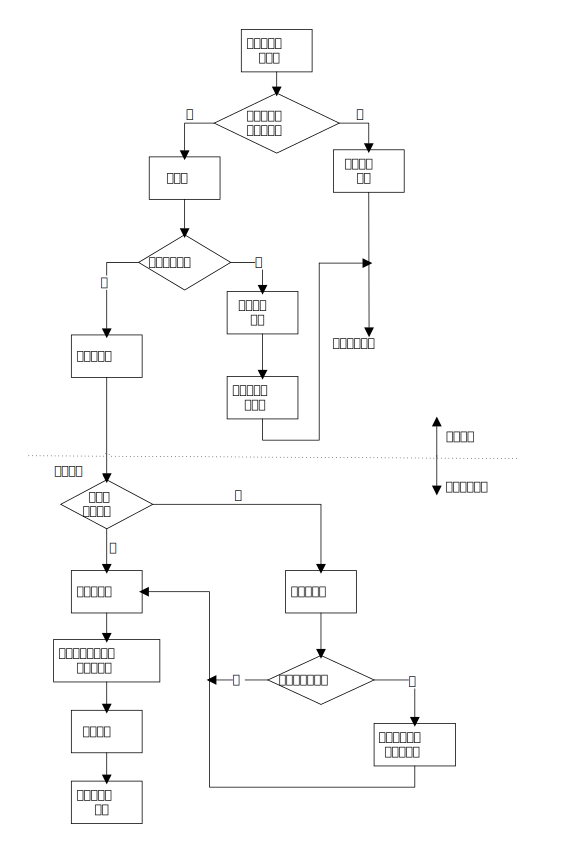
\includegraphics[width=0.8\textwidth]{img/3.3.4.1}
		\end{figure}
		\begin{itemize}
			\item 主存驻留标志:记录该页是否驻存在主存中
			\item 写回标志:记录该页在主存中有无被修改,当该页需要从主存淘汰,且如果该页被修改,则需要写回磁盘
			\item 保护标志:记录该页的保护属性,供共享保护使用
			\item 引用标志:记录该页的引用情况,供页面淘汰算法使用
			\item 可移动标志:记录该页是否可以移动,正在与外设交换的页面是不能被移动的
		\end{itemize}
		页式虚拟存储管理的地址转换
		\begin{figure}[H]
			\centering
			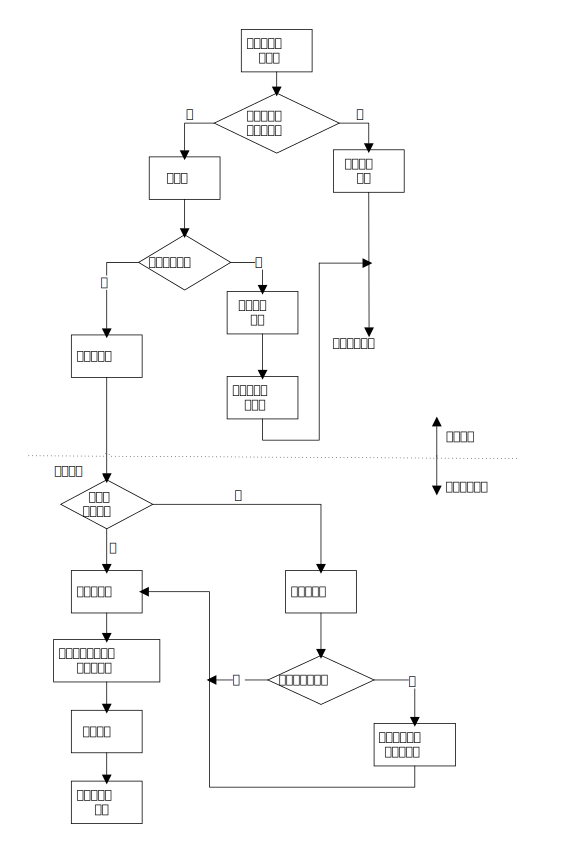
\includegraphics[height=0.55\textheight]{img/3.3.4}
		\end{figure}

		TLB、page、cache 的缺失组合情况
		\begin{table}[H]
			\centering
			\begin{tabular}{|c|c|c|c|c|}
				\hline
				序号 & TLB  & page & cache & 说明                                   \\ \hline
				1  & hit  & hit  & hit   & 可能,TLB 命中则页一定命中,信息在主存,就可能在 cache 中   \\ \hline
				2  & hit  & hit  & miss  & 可能,TLB 命中则页一定命中,信息在主存,但可能不在 cache 中  \\ \hline
				3  & miss & hit  & hit   & 可能,TLB 缺失但页可能命中,信息在主存,就可能在 cache 中   \\ \hline
				4  & miss & hit  & miss  & 可能,TLB 缺失但页可能命中,信息在主存,但可能不在 cache 中  \\ \hline
				5  & miss & miss & miss  & 可能,TLB 缺失,则页也可能缺失,信息不在主存,一定也不在 cache \\ \hline
				6  & hit  & miss & miss  & 不可能,页缺失,说明信息不在主存,TLB 中一定没有该页表项       \\ \hline
				7  & hit  & miss & hit   & 不可能,页缺失,说明信息不在主存,TLB 中一定没有该页表项       \\ \hline
				8  & miss & miss & hit   & 不可能,页缺失,说明信息不在主存,cache 中一定也没有该信息     \\ \hline 
			\end{tabular}
		\end{table}

		\subsection{页面调度}
		页面调度是指当主存空间已满而又需要装入新页时,页式虚拟存储管理必须按照一定的算法把已在主存的一些页调出去
		\begin{itemize}
			\item 选择淘汰页的工作称为页面调度,选择淘汰页的算法称为页面调度算法
			\item 页面调度算法设计不当,会出现频繁的调入/调出,这种现象称为抖动或颠簸
		\end{itemize}
		衡量存储管理性能和用户编程水平的重要依据——缺页中断率
		\begin{itemize}
			\item 假定进程 $P$ 共 $n$ 页,此进程分得页框 $m$ 个
			\item 进程 $P$ 运行中成功访问次数为 $S$,不成功访问次数为 $F$,总访问次数 $A=S+F$
			\item 定义缺页中断率  $f=F/A$
			\item 影响缺页中断率的因素:
			\begin{itemize}
				\item 分配给进程的页框数:可用页框数越多,则缺页中断率就越低
				\item 页面的大小:页面尺寸越大,则缺页中断率就越低
				\item 页面替换算法:算法的优劣影响缺页异常次数
				\item 程序特性:程序局部性要好,它对缺页中断率有很大影响
			\end{itemize}
		\end{itemize}
		\textbf{例}:与程序设计有关的缺页中断率
		\begin{figure}[H]
			\centering
			\includegraphics[width=0.8\textwidth]{img/3.3.5}
		\end{figure}

		下面讨论页面调度算法
		\subsubsection{最佳置换OPT页面调度算法}
		\begin{itemize}
			\item 算法描述:当要调入新页面时,首先淘汰以后不再访问的页,如果没有这样的页,就选择\textbf{距现在最长时间后再访问}的页
			\item 该方法由 Belady 提出,又称为 Belady 算法
			\item OPT 只可以\textbf{模拟},不可以实现,因为永远无法预知之后的事情
			\item 这种算法可以用作衡量其他各种算法的标准
		\end{itemize}
		\begin{figure}[H]
			\centering
			\includegraphics[width=0.9\textwidth]{img/OPT}
		\end{figure}

		\subsubsection{先进先出FIFO页面调度算法}
		\begin{itemize}
			\item 算法描述:首先淘汰最先调入主存的那一页,或者说主存驻留时间最长的那一页(常驻的除外)
			\item 模拟的是程序执行的顺序性,有一定合理性,并不能很好模拟程序的循环性
		\end{itemize}
		\begin{figure}[H]
			\centering
			\includegraphics[width=0.9\textwidth]{img/FIFO}
		\end{figure}
		FIFO 算法的 Belady 异常:更多的页框导致了更高的缺页率
		\begin{figure}[H]
			\centering
			\includegraphics[width=0.9\textwidth]{img/Belady异常}
		\end{figure}

		\subsubsection{最近最少使用LRU页面调度算法}
		\begin{itemize}
			\item 算法描述:淘汰\textbf{最近一段时间较久未被访问}的那一页,即那些刚被使用过的页面,可能马上还要被使用到
			\item 模拟了程序执行的局部属性,既考虑了\textbf{循环性},又兼顾了\textbf{顺序性}
			\item 严格实现的代价大,需要维护页面淘汰队列,实现起来相当困难,所以只能模拟
		\end{itemize}
		\begin{figure}[H]
			\centering
			\includegraphics[width=0.9\textwidth]{img/LRU}
		\end{figure}

		LRU 算法的模拟实现\footnote{该模拟相当不严谨,它并未模拟出一个淘汰的序列,而是简单地将页面分为两类,所以只是一个非常粗糙的模拟}
		\begin{itemize}
			\item 为每个主存驻留页建一个引用标志位供硬件使用
			\item 设置一个时间间隔中断,中断发生时,所有驻留页的引用标志位置为 0,而地址转换时,引用标志位置为 1
			\item 在淘汰页面时只需要从引用标志位为 0 的页面中随机淘汰一个即可
			\item 该算法的难点是时间间隔的长度如何设置,太短则全是 0,太长则全是 1,就退化为随机调度了
		\end{itemize}

		\subsubsection{最不常使用LFU页面调度算法}
		\begin{itemize}
			\item 算法描述:淘汰最近一段时间内\textbf{访问次数较少}的页面
			\item 对 OPT 的模拟性比 LRU 更好
			\item 基于时间间隔中断,并给每一页设置一个计数器,时间间隔中断发生后,所有计数器清 0,每访问页一次就给计数器加 1,选择计数最小的页面淘汰
		\end{itemize}

		\subsubsection{时钟CLOCK页面调度算法}
		采用循环队列机制构造页面队列,形成了一个类似于钟表面的环形表
		\begin{itemize}
			\item 队列指针则相当于钟表面上的表针,指向可能要淘汰的页面
			\item 使用页引用标志位
		\end{itemize}
		\begin{figure}[H]
			\centering
			\includegraphics[width=0.9\textwidth]{img/clock}
		\end{figure}
		CLOCK 算法的工作流程
		\begin{itemize}
			\item 页面调入主存时,其引用标志位置为 1
			\item 访问主存页面时,其引用标志位置为 1
			\item 淘汰页面时,从指针当前指向的页面开始扫描循环队列
			\begin{itemize}
				\item 把所遇到的引用标志位是 1 的页面的引用标志位清 0 并跳过
				\item 把所遇到的引用标志位是 0 的页面淘汰,指针推进一步
			\end{itemize}
		\end{itemize}
		\begin{figure}[H]
			\centering
			\includegraphics[width=0.9\textwidth]{img/3.3.5.5}
		\end{figure}


		\subsubsection{不同算法性能比较}
		\begin{figure}[H]
			\centering
			\includegraphics[width=0.65\textwidth]{img/3.3.5.6}
		\end{figure}
		这是一个整体性能的比较,对于个例,有可能 CLOCK 优于 LRU

		\subsection{反置页表}
		一些计算机系统使用反置页表来实现页式虚拟存储管理的地址管理,为此专门设置了\textbf{主存管理单元}(memory management unit, MMU)
		\begin{itemize}
			\item 它是处理器管理虚拟/物理存储器的控制电路,完成把虚拟地址映射为物理地址的任务,并提供存储保护,必要时确定淘汰页面
			\item 主存管理单元要用到一个关键性的数据结构——反置页表 (inverted page table, IPT)
		\end{itemize}

		反置页表是针对主存页框建立的一个页表,它的页表项按照页框号排序
		\begin{itemize}
			\item 其表项包括正占有该页框的进程号/页号、特征位和哈希链指针等
			\item 用来完成内存页架到访问进程页号的对应,即物理地址到逻辑地址的转换
		\end{itemize}

		反置页表的页表项
		\begin{itemize}
			\item 页号:虚拟地址页号
			\item 进程标志符:使用该页的进程号(页号和进程标志符结合起来标志一个特定进程的虚拟地址空间的一页)
			\item 标志位:有效、引用、修改、保护和锁定等标志信息
			\item 链指针:哈希链,如果某个项没有链项,则该域为空(允许用一个单独的位来表示)
		\end{itemize}
		\begin{figure}[H]
			\centering
			\includegraphics[width=0.65\textwidth]{img/3.3.6}
		\end{figure}
		上图未显示选择淘汰页面,该功能同样由 MMU 完成

		基于反置页表的地址转换过程
		\begin{itemize}
			\item MMU 通过哈希表把进程标识和虚页号转换成一个哈希值,指向 IPT 的一个表目
			\item MMU 遍历哈希链找到所需进程的虚页号,该项的索引就是页架号,通过拼接位移便可生成物理地址
			\item 若遍历整个反置页表中未能找到匹配页表项,说明该页不在内存,产生缺页中断,请求操作系统调入
		\end{itemize}

		\textbf{例:}线性反置页表和哈希线性反置页表
		\begin{figure}[H]
			\centering
			\includegraphics[width=0.95\textwidth]{img/3.3.6.1}
		\end{figure}


		\section{段式存储管理}
		\subsection{段式程序设计}
		高级语言采用模块化程序设计方法
		\begin{itemize}
			\item 应用程序由若干程序段(模块)组成
			\begin{itemize}
				\item 如由主程序段(M)、子程序段(X)、数据段(D)和工作区段(W)组成
			\end{itemize}
			\item 每一段都从 0 开始编址,各有各自名字和长度且实现不同功能
			\item 编译后段间地址是不连续的,段内地址是连续的
		\end{itemize}
		\begin{figure}[H]
			\centering
			\includegraphics[width=0.6\textwidth]{img/3.4.1.1}
		\end{figure}

		\subsubsection{段式存储管理}
		分段存储器的逻辑地址由两部分组成:段号 + 段内偏移,段式存储管理中段的划分对程序员可见

		\textbf{例:}段式存储管理中物理地址和逻辑地址之间的转换
		\begin{figure}[H]
			\centering
			\subfloat[]{
				\includegraphics[width=0.35\textwidth]{img/3.4.1.2.1}
			}
			\subfloat[]{
				\includegraphics[width=0.6\textwidth]{img/3.4.1.2.2}
			}
		\end{figure}

		段式存储管理基于可变分区存储管理实现,一个进程要占用多个分区

		硬件需要增加一组用户可见的段地址寄存器(代码段、数据段、堆栈段,附加段)供地址转换使用

		存储管理需要增加设置一个段表,每个段占用一个段表项
		\begin{itemize}
			\item 包括:段始址、段限长,以及存储保护、可移动、可扩充等标志位
		\end{itemize}

		段式存储管理的地址转换流程
		\begin{figure}[H]
			\centering
			\includegraphics[width=0.5\textwidth]{img/3.4.1.2.3}
		\end{figure}

		\subsubsection{段的共享}
		\begin{itemize}
			\item 通过不同进程段表中的项指向同一个段基址来实现段的共享
			\item 对共享段的信息必须进行保护,如规定只能读出不能写入,不满足保护条件则产生保护中断
			\item 为了方便共享,系统中常常建立一张共享段表记录所有共享段,包含段名、共享计数、段长、段首址、保护位等
		\end{itemize}

		\subsection{段式虚拟存储管理}
		\subsubsection{段式虚拟存储管理的基本思想}
		把进程的所有分段都存放在辅存中,进程运行时先把当前需要的一段或几段装入主存,在执行过程中访问到不在主存的段时再把它们动态装入

		段式虚拟存储管理中段的调进调出是由操作系统自动实现的,对用户透明

		与段覆盖技术不同,它是用户控制的主存扩充技术,操作系统不感知

		\subsubsection{段式虚拟存储管理的段表}
		段式虚拟存储管理需要对段表进行扩充
		\begin{itemize}
			\item 既要包括普通段表中主存的基址/限长,还要有辅存的位置
			\item 同时标志位也要进行扩充。主要有以下一些标志位:
			\begin{itemize}
				\item 特征位:表示是否在主存或共享段
				\begin{itemize}
					\item 00(不在内存)、01(在内存)、11(共享段)
				\end{itemize}
				\item 存取权限位:表示是否可执行、可读、可写
				\begin{itemize}
					\item 00(可执行)、01(可读)、11(可写)
				\end{itemize}
				\item 扩充位:表示段长度是否能动态扩充
				\begin{itemize}
					\item 0(固定长)、1(可扩充)
				\end{itemize}
				\item 标志位:表示是否修改过、是否可以移动
				\begin{itemize}
					\item 00(未修改)、01(已修改)、11(不可移动)
				\end{itemize}
			\end{itemize}
		\end{itemize}
		\begin{figure}[H]
			\centering
			\includegraphics[width=0.9\textwidth]{img/3.4.2.2}
		\end{figure}

		\subsubsection{段式虚拟存储管理的地址转换与存储保护}
		\begin{figure}[H]
			\centering
			\includegraphics[width=0.9\textwidth]{img/3.4.2.3}
		\end{figure}

		\subsection{段页式存储管理}
		\subsubsection{段页式存储管理}
		段页式存储管理的基本思想
		\begin{itemize}
			\item 段式存储管理可以基于页式存储管理实现
			\item 每一段不必占据连续的存储空间,可存放在不连续的主存页架中
			\item 能够扩充为段页式虚拟存储管理
			\item 装入部分段,或者装入段中部分页面
		\end{itemize}

		段页式存储管理的段表和页表
		\begin{figure}[H]
			\centering
			\includegraphics[width=0.6\textwidth]{img/3.4.3.1.1}
		\end{figure}

		段页式存储管理的地址转换
		\begin{figure}[H]
			\centering
			\includegraphics[width=0.75\textwidth]{img/3.4.3.1.2}
		\end{figure}

		\subsubsection{段页式虚拟存储管理}
		段页式虚拟存储基本原理
		\begin{itemize}
			\item 虚地址以程序的逻辑结构划分为段,这是段页式的段式特征
			\item 实地址划分层位置固定、大小相同的页框(块),这是段页式的页式特征
			\item 将每一段的线性地址空间划分成与页框大小相同的页面,这是段页式的特征
			\item 逻辑地址由段号 $s$、段内页号 $p$ 和页内偏移 $d$ 组成
			\begin{itemize}
				\item 对用户来说,虚拟地址由段号 $s$ 和段内位移 $d^\prime$ 组成
				\item 系统内部将 $d^\prime$ 分解为 $p$ 和 $d$,且 $d^\prime = p \times \mbox{块长} + d$
			\end{itemize}
			\item 请求段页式虚拟存储管理的数据结构比较复杂,包含作业表、段表和页表三部分
			\begin{itemize}
				\item 作业表:进入系统的作业和作业段表的起始地址
				\item 段表:是否在内存、段页表起始地址
				\item 页表:是否在内存、对应内存块号
			\end{itemize}
		\end{itemize}

		段页式虚拟存储管理的地址转换
		\begin{figure}[H]
			\centering
			\includegraphics[width=0.75\textwidth]{img/3.4.3.2}
		\end{figure}

\end{document}



